% !TeX root = ../master.tex

\lecture{1}{2026-08-27}{Course Outline and Introduction}

\section{Introduction}

\subsection{What is Manufacturing}
As a technological process, manufacturing is the application of a physical and/or chemical process to alter the geometry, properties, and/or appearance of a starting material to make parts or products.
Economically, a manufacturing process can be seen as the transformation of materials into items of greater value by one or more processing and/or assembly operations.

\subsection{Production Quantity and Product Variety}
The \textit{Production Quantity} $Q$ is the quantity of products made by a factory.
Annual quanitites are classified into three ranges:
\begin{itemize}
  \item Low Production --- 1--100 units
  \item Medium Production --- 100--\num{10000} units
  \item High/Mass Production --- \num{10000}+ units
\end{itemize}

The \textit{Product Variety} $P$ refers to different product types or models produced in the plant.
These different products often have different features, are intended for different markets, or have different parts.
The number og different product types made each year in a factory can be counted yielding the product variety of that year. 

Although product variety $P$ is quantitative, it is much less exact than the production quantity $Q$ because details on how much the designs differ is not captured accurately simply by the number of different designs.
If the difference between products is small it is termed \textit{Soft Product Variety} (e.g. storage options on a PC) and if the products differ substantially it is termed \textit{Hard Product Variety} (e.g. a car company producing both semi-trucjs and small cars).

\subsection{Manufacturing Capability and Processes}
Manufacturing capability is a measure of how ``much'' manufacturing is possible.
This depends on both technological process capability, physical product limitations, or limited production capacity. 

Material parameters are of high importance here.
Most materials can be classified as either metals, ceramics, composites, or polymers.
Each have different chemistry meaning their mechanical and physical properties are different.

Different manufacturing processes can be classified as shown on \mref{fig:classification}.
The main focuses of this course will be on the shaping processes and permanent joining.

\begin{figure} [ht]
  \centering
  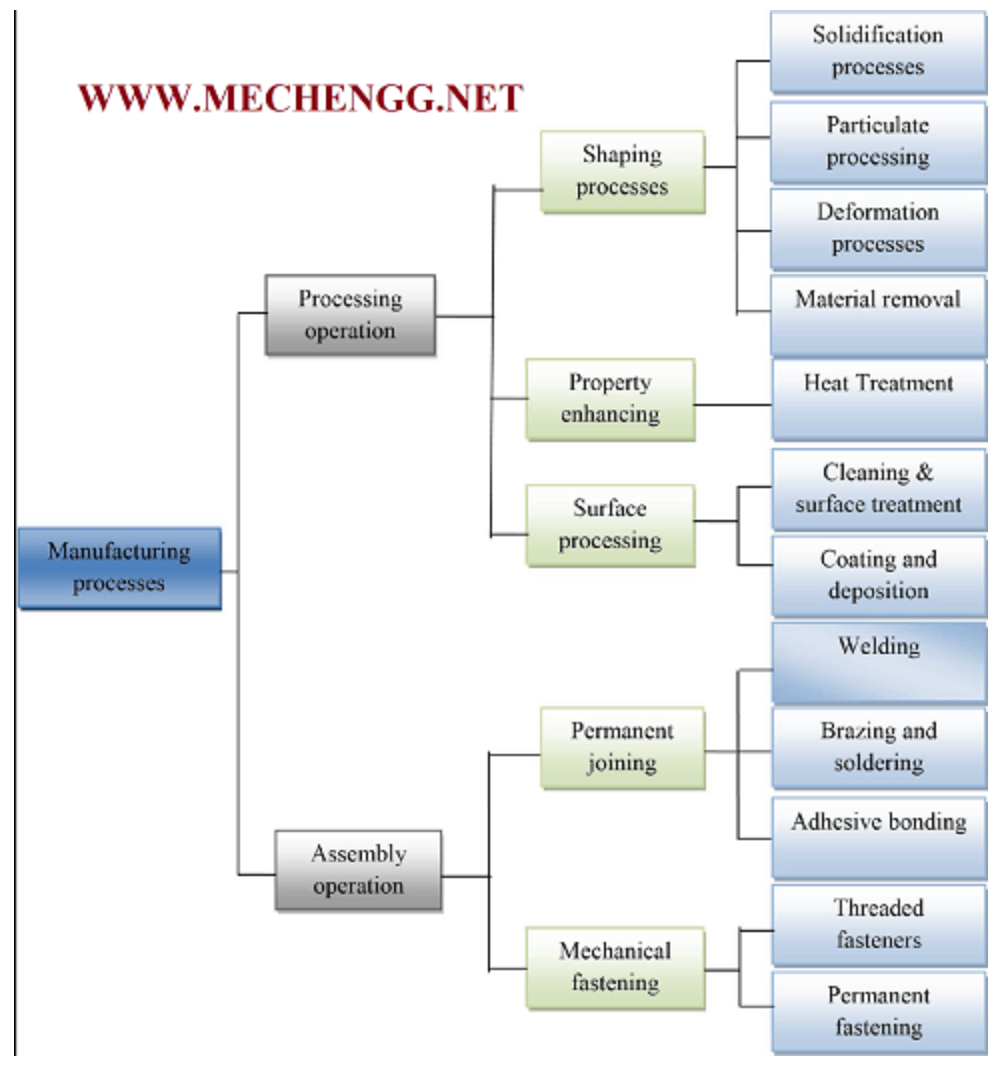
\includegraphics[width=0.5\linewidth]{./figures/classification.png}
  \caption{Classification of manufacturing processes \parencite{introductionmanufacturingprocesses}}
  \label{fig:classification}
\end{figure}


\subsection{Manufacturing Production Systems}
Product development normally follows a so-called ``S''-curve, where the performance starts of at a low point before growing quickly until the product has matured or the design has been optimized sufficiently that the increase in performance will wane off.
This looks a bit like the sigmoid function, if performance is plotted with respect to time invested.

A production system may follow the model shown on \mref{fig:modelprodsys}.
\begin{figure} [ht]
  \centering
  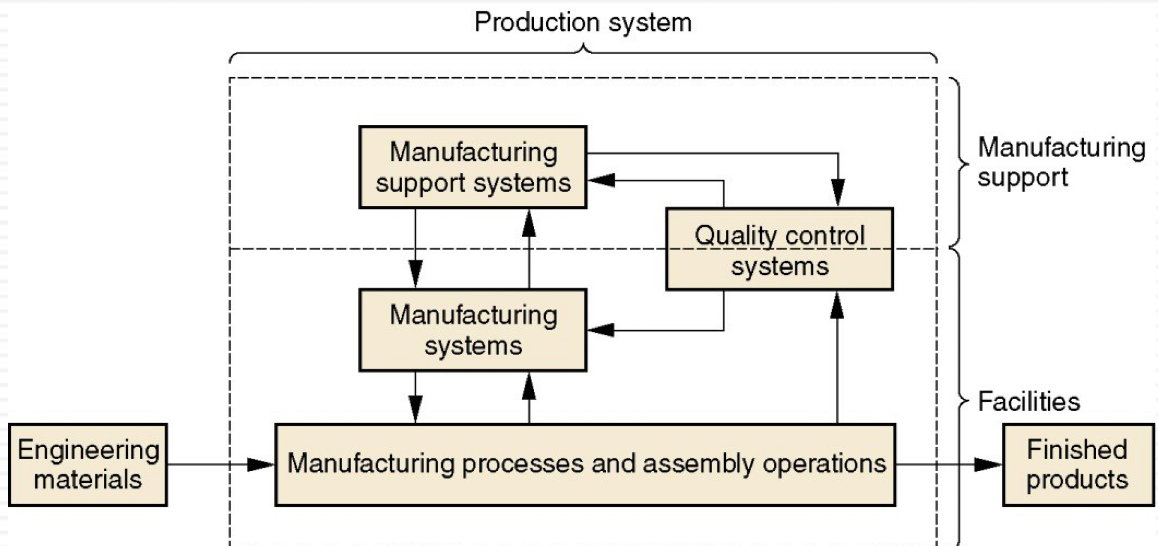
\includegraphics[width=0.8\linewidth]{./figures/modelprodsys.png}
  \caption{Model of a production system}
  \label{fig:modelprodsys}
\end{figure}
Many factors here are able to be changed, e.g.
\begin{itemize}
  \item Product design
  \item Materials
  \item Labor costs
  \item Equipment
  \item Manufacturing costs
\end{itemize}

\subsubsection{Low Production}
Low Production systems are sometimes called \textit{Job shops}.
These job shops makes low quantities of specialized and highly-customized products, e.g. space capsules, prototype aircraft, special machinery, etc.
The equipment at these places is general purpose but the labor force is highly skilled meaning job shops offer maximal flexibility.

\subsubsection{Medium Production}
Two different types of facility exists, depending on product variety.
For medium to hard product variety, \textit{batch production} is often used, where different setups are required between batches.
For soft variety plants, \textit{Cellular Manufacturing} is widespread.
Here, worker cells are organized to process parts without setups between different part styles.

\subsubsection{High Production}
Also called \textit{mass production}, this type of production is needed when the demand for product is high and the entire manufacturing system is dedicated to the production of that product.
This also exists in two categories.
The first is \textit{Quantity Production}, i.e. mass production of single parts on a single or small number of machines, and the second is \textit{Flow Line Production}, i.e. multiple machines or workstations arranged in sequence, as in a production line.
